\documentclass[12pt,letterpaper]{article}
\usepackage[utf8]{inputenc}
% AMS packages
\usepackage{amsmath}
\usepackage{amsfonts}
\usepackage{amssymb}
% no indent at new paragraph
\usepackage[parfill]{parskip}
% to include figures 	
\usepackage{graphicx}
% for consistent SI units
\usepackage{siunitx}
\sisetup{%
  output-decimal-marker={.},
  load-configurations=abbreviations,
  %group-separator={,},
  sticky-per=true,
  %per-mode=fraction
  per-mode=symbol
}
% to hyperlink figure and equation numbers in a pdf
\usepackage[colorlinks=false, pdfborder={0 0 0}]{hyperref}
\usepackage{bigints}
\usepackage{relsize}
\begin{document}

\title{Simulating Laminar Flow over a Flat Plate with an Isothermal Wall in SU2}
\author{Kedar R. Naik \\
 Stanford University \\
 \texttt{knaik@stanford.edu}}
\date{\today}
\maketitle

\begin{abstract}
Several simulations of flat-plate flow were performed using SU2 at NASA Glenn from June to July of 2014. Here, one specific case has been investigated again, namely: laminar flow over a flat plate with an isothermal wall boundary condition. The temperature difference between the freestream and the surface is relatively small compared to the previous simulations. Moreover, a low freestream Mach number has been chosen in an attempt to minimize the effects of compressibility. Various quantities of interest from this new simulation have been plotted. When appropriate, computational results are compared with analytical solutions. The purpose of this report is to assist work on thermal boundary layers that is currently ongoing at NASA Glenn.
\end{abstract}

\section*{Preliminaries}
The physical flow parameters of this simulation as well as the numerical methods used have been described below.

\subsection*{Flow Conditions}
The case run simulates the laminar flow of air ($\gamma$ = 1.4) over a flat plate held at a constant temperature, $T_w$. Specific conditions of the flow are listed below.

\begin{align*}
&c_p = \SI{1005}{\joule\per\kilogram\kelvin} & \text{specific heat capacity} \\
&k = \SI{0.02618}{\watt\per\meter\kelvin} & \text{thermal conductivity} \\
&p_{t_{in}} = \SI{100000}{\pascal} & \text{inlet stagnation pressure} \\
&p_{out} = \SI{99303.1}{\pascal} & \text{outlet static pressure} \\
&Pr = 0.72 &\text{Prandtl number} \\
&T_{t_{in}} = \SI{300}{\kelvin} & \text{inlet stagnation temperature} \\
&T_w = \SI{350}{\kelvin} & \text{isothermal wall temperature} \\
&T_\infty = \SI{300}{\kelvin} & \text{freestream temperature} \\
&U_\infty = \SI{34.7715}{\meter\per\second} & \text{freestream velocity}\\
&\mu = \SI{1.84492e-5}{\newton\second\per\meter\squared} & \text{dynamic viscosity} \\
&\rho_\infty = \SI{1.13753}{\kilogram\per\meter\cubed} & \text{freestream density}
\end{align*}

N.B. The static pressure at the outlet, $p_{out}$, was computed using the isentropic relation

\begin{equation*}
p_{out} = p_{t_{in}}\left[ 1+\dfrac{1}{2}\left( \gamma-1\right) M_\infty^2 \right] ^{-\dfrac{\gamma}{\left( \gamma-1\right) }}.
\end{equation*}

A low freestream Mach number of $M_\infty$ = 0.1 was selected to minimize the effects of compressibility.

\subsection*{Numerical Methods}
The Navier-Stokes equations without a turbulence model were used to model laminar flow. The specific algorithms and relaxation schemes used to solve the problem are listed below.

\begin{description}
\item[CFL number on finest grid:] 3.0
\item[linear solver:] FGMRES
\item[linear solver preconditioner:] LU-SGS
\item[multigridding levels:] 1
\item[convective scheme:] Roe, $2^{nd}$-order
\end{description}

\section*{Results}
Some salient results from the simulation done in SU2 are presented here. This includes evidence of numerical convergence as well as extracted profiles of skin friction, temperature, and Nusselt number.

\subsection*{Numerical Convergence}
The problem was considered to be converged after seeing the residual in density fall five orders of magnitude. A plot of the residual history is found in Fig.~\ref{fig:rho_res}.

\begin{figure}[h] 
\centering
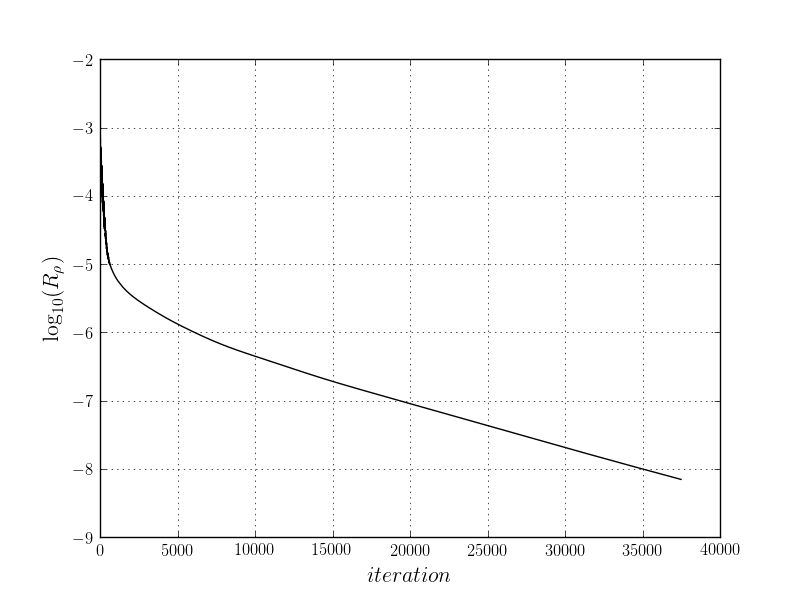
\includegraphics[width=\linewidth]{rho_residual.png}
\caption{Convergence history of the density residual, $R(\rho)$.}
\label{fig:rho_res}
\end{figure}

\subsection*{Skin Friction}
Fig.~\ref{fig:cf} compares the coefficient of skin friction, $C_f$, calculated by SU2 with that of the analytical solution by Blasius:

\begin{equation*}
C_f(x) = \dfrac{0.6641}{\sqrt{Re_x}}.
\end{equation*}

Checking the skin friction coefficient is generally a good way of assessing the quality of a laminar, flat-plate simulation.

\begin{figure}[h] 
\centering
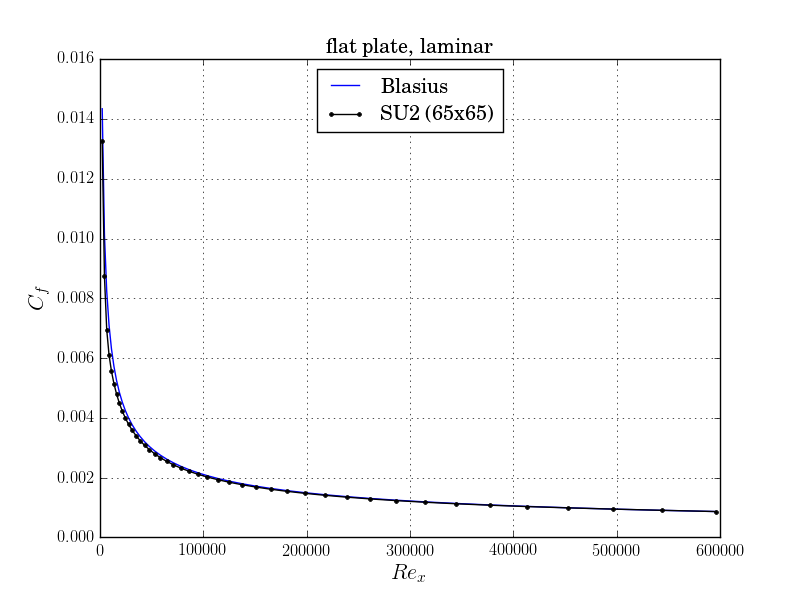
\includegraphics[width=\linewidth]{cf_350.png}
\caption{Variation in $C_f$ along the length of the plate.}
\label{fig:cf}
\end{figure}

\subsection*{Thermal Boundary Layer}
The isothermal wall condition allows one to investigate the development and growth of thermal boundary layers along the surface of the plate. In Fig.~\ref{fig:temp}, nondimensionalized temperature along the outlet boundary (i.e. at the end of the plate), 

\begin{equation*}
\theta = \dfrac{T-T_w}{T_\infty-T_w},
\end{equation*}

has been plotted against nondimensionalized wall distance,

\begin{equation*}
\eta = \dfrac{y}{\sqrt{\dfrac{\nu x}{U_\infty}}},
\end{equation*}

where $\nu = \mu/\rho$ denotes the kinematic viscosity.

The temperature profile extracted from the SU2 output is also compared against the analytical solution of Pohlhausen as well as the Crocco-Busemann relation, which is designed to account for the effects of compressibility. Pohlhausen's solution is given by

\begin{equation*}
\theta_{Pohlhasusen} = 1 - \dfrac{\mathlarger{\mathlarger{\int_{\eta}^{\infty}}}\left( \dfrac{d^2f}{d\eta^2}\right)^{Pr}d\eta}{\mathlarger{\mathlarger{\int_{0}^{\infty}}}\left( \dfrac{d^2f}{d\eta^2}\right)^{Pr}d\eta}
\end{equation*}

\begin{figure}[h] 
\centering
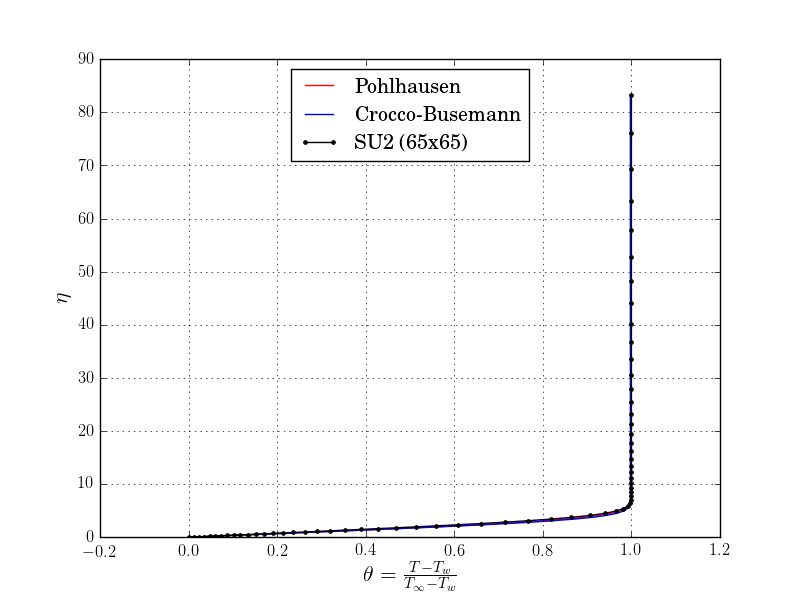
\includegraphics[width=\linewidth]{temp_350.png}
\caption{Nondimensionalized temperature profile at the outlet.}
\label{fig:temp}
\end{figure}

\end{document}